\documentclass[12pt, oneside]{article}   	% use "amsart" instead of "article" for AMSLaTeX format
\usepackage{lipsum}% http://ctan.org/pkg/lipsum
\usepackage{xcolor}% http://ctan.org/pkg/xcolor
\usepackage{fancyhdr}% http://ctan.org/pkg/fancyhdr
\usepackage{geometry}                		% See geometry.pdf to learn the layout options. There are lots.
\geometry{letterpaper}                   		% ... or a4paper or a5paper or ... 
\usepackage[parfill]{parskip}    		% Activate to begin paragraphs with an empty line rather than an indent
\usepackage{graphicx}				% Use pdf, png, jpg, or eps§ with pdflatex; use eps in DVI mode
\usepackage{amssymb}
\usepackage{subfig}
\usepackage{float}
\usepackage{caption}
\usepackage[some]{background}



%----------------------------------------------------------------------------------------
%	DEFINE COLOR
%----------------------------------------------------------------------------------------
\definecolor{myBlue}{RGB}{16, 137, 141}

%----------------------------------------------------------------------------------------
%	SECTION LINE
%----------------------------------------------------------------------------------------
\usepackage{titlesec}
\titleformat{\section}
{\Large\sffamily}
{\thesection.}{.5em}{}[\color{myBlue}\titlerule]

\titleformat{\subsection}{\large\sffamily}
\titleformat{\subsubsection}{\sffamily}





%----------------------------------------------------------------------------------------
%	TITLE PAGE
%----------------------------------------------------------------------------------------

\definecolor{titlepagecolor}{cmyk}{1,.60,0,.40}

\DeclareFixedFont{\bigsf}{T1}{phv}{b}{n}{1.5cm}

\backgroundsetup{
scale=1,
angle=0,
opacity=1,
contents={\begin{tikzpicture}[remember picture,overlay]
 \path [fill=myBlue] (-0.5\paperwidth,5) rectangle (0.5\paperwidth,10);  
\end{tikzpicture}}
}
\makeatletter                       
\def\printauthor{%                  
    {\large \@author}}              
\makeatother
\author{%
    Elsa Bergman \\     Angelica Elvin  \\  Anna Eriksson   \\ Arvid Gr\"{a}ns \\ Frida Korns\"{a}ter \\ Frans Larsson  \\       Therese Olsson
    }


%----------------------------------------------------------------------------------------
%	HEADER AND FOOTER
%----------------------------------------------------------------------------------------

\fancypagestyle{myheader}{%
  \fancyhf{}% Clear all headers/footers
  \fancyhead[C]{Deliverable II $|$ \textit{@Campus}}% Header Centred
  \fancyfoot[C]{\thepage}% Footer Centred
  \renewcommand{\headrulewidth}{2pt}% 2pt header rule
  \renewcommand{\headrule}{\hbox to\headwidth{%
    \color{myBlue}\leaders\hrule height \headrulewidth\hfill}}
  \renewcommand{\footrulewidth}{0pt}% No footer rule
}
\setlength{\headheight}{21pt}%

%----------------------------------------------------------------------------------------
%	BEGIN DOCUMENT 
%----------------------------------------------------------------------------------------
\begin{document} 
\begin{titlepage}
\BgThispage
\newgeometry{left=1cm,right=4cm}
\vspace*{2cm}
\noindent
\textcolor{white}{\Huge{\textbf{Deliverable II}}} \\
\\
\textcolor{white}{\Large Requirements of the smartphone application \textit{@Campus}}
\vspace*{2.5cm}\par
\noindent
\begin{minipage}{0.35\linewidth}
    \begin{flushright}
        \printauthor
    \end{flushright}
\end{minipage} \hspace{15pt}
%
\begin{minipage}{0.02\linewidth}
    \rule{1pt}{175pt}
\end{minipage} \hspace{-10pt}
%
\begin{minipage}{0.6\linewidth}
\vspace{5pt}
	\renewcommand{\abstractname}{Introduction}
    \begin{abstract} 
\noindent The purpose of this deliverable is to describe the requirements of the application \textit{@Campus}. It will include both functional and non-functional requirements of the system, the overall design and the expected users. 
    \end{abstract}
\end{minipage}
\end{titlepage}
\restoregeometry

\pagestyle{myheader}




%\date{}							% Activate to display a given date or no date

\newpage
\section{Overview of the system}
The smartphone application \textit{@Campus} is a system designed for Android phone. The purpose of the application is to collect events happening on different Uppsala university campuses. The events could include free coffee handouts by companies, lunch lectures or promotion of events arranged by the Student Union. The first goal is to make the application functional for the �ngstr�m and ITC campus, with extensions to all campuses of Uppsala University if there is time. In the application, the user can log in as either admin, organizations or student to be able to use the application. Both users have similar view but there are some features that differ. 

For a student account, the user can view ongoing events at his/her selected campuses, view upcoming events and save events to favorites. In addition to this, there will also be a live feed where student users view and add happenings/information in an informal way e.g. "Free coffee at �ngstr�ms today", "STS is wonderful" or "Sveriges ingenj\"{o}rer hand out fancy pencils today, wow". The purpose of the live feed is that users can easily connect to each other and in a quick and spontaneous way inform other users about events going on right now. 

For an organization account, the major feature is to add events to the application. Therefore an organization account will have an extra option in the menu called "Add Event" where the user can create an event and fill in the information. When an event has been created, the admin has to approve the event in order for the event to appear in the application. 

For an admin account, the admin has all the features and functionality that a student user has with the addition of an admin-page where the admin can view all users and edit or remove a user. An admin can also remove comments in the live feed and approve events (and modify events if needed). If an admin removes or modifies an event, the creator of the event will receive a notification with an explanation from the admin regarding why the event was deleted or modified. 

An overview of the design in progress is given in figure \ref{design}. 

\begin{figure}[H]
  \centering
  \subfloat[First page.]{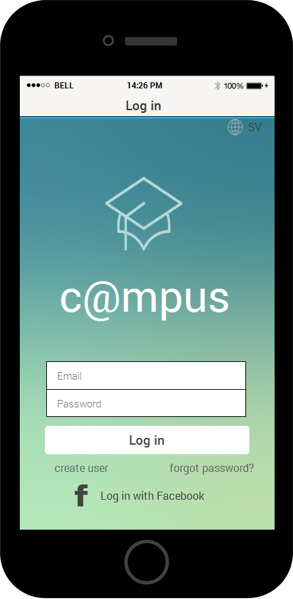
\includegraphics[scale=0.8]{login.png}\label{w=0.2}}
  \hfill
  \subfloat[Toggle menu for admin.]{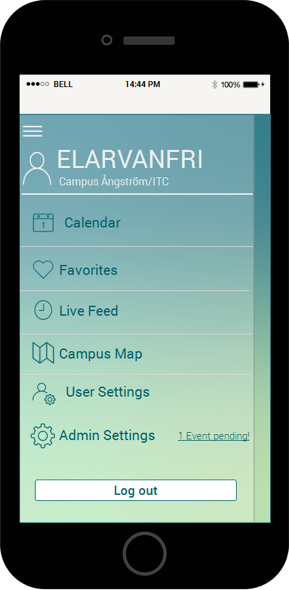
\includegraphics[scale=.8]{menu.png}\label{w=1}}
    \hfill
  \subfloat[Livefeed for users.]{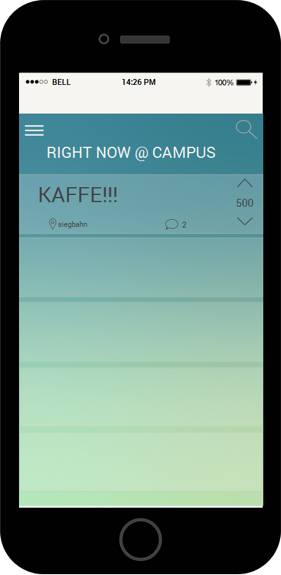
\includegraphics[scale=.8]{flow.png}\label{w=2.16}}
    \hfill
  \subfloat[Create user.]{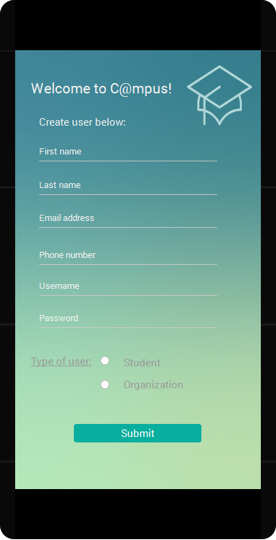
\includegraphics[scale=.8]{signup.png}\label{w=3}}
    \hfill
  \subfloat[Profile page for organizations.]{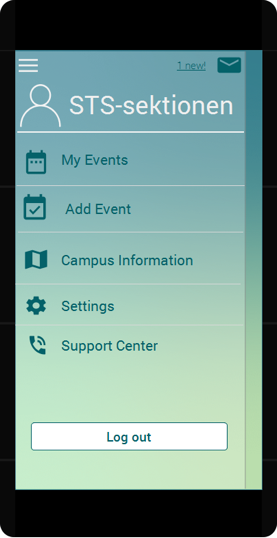
\includegraphics[scale=.8]{profile.png}\label{w=4}}
    \hfill
  \subfloat[My events for organizations.]{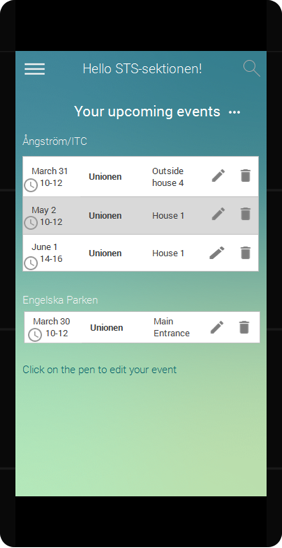
\includegraphics[scale=.8]{events.png}\label{w=5}}
    \hfill
  \caption{}
  \label{design}
\end{figure} 

\section{Overview of the expected users}
The expected target group of \textit{@Campus} is students and exchange student at Uppsala University, but both students and organizations can use the app. These kinds of users have different features where students can add small events in the live feed compared to the organizations that can add a bigger events to the calendar. In addition to these users there will also be administrators which will approve the events.

Today Facebook is a platform used by many organizations to broadcast events. We therefore believe that this app, which do not require Facebook, is highly relevant for users with no Facebook account. Even if you have Facebook you need to have the "right" social network to get an invite to a Facebook-event and this is a problem that doesn't exist in the application \textit{@Campus}. 

\section{Financing}
A way to make a profit of the application is to charge the organizations in exchange of  boosting their specific event or highlighting their event in the app. This is similar to Google's search engine where companies can pay to have their webpage at the top of the search result. Another way to make money is to have relevant ads in the application such as restaurants or coffee shops which are located at the campus. A future development when \textit{@campus} is established is that the organization has to pay to have an account in order to promote their events in the app. 

\section{List of non-functional and functional requirements}
\subsection*{Non-functional requirements}
\begin{itemize}
\item The system \textit{is} an Android smartphone application.
\item A person \textit{must} be a registered user to be able to interact with the app. 
\item An event \textit{will} disappear from the application view after the event has finished. This \textit{could} be solved by having a timer which decides when to remove it. 
\item The system \textit{must} have a high degree of usability for both users, admins and non-logins. 
\item The system \textit{must} have high degree of security for both users and admins. This concerns user information such as usernames, email and passwords. 
\item There are three user-roles: student-user, admin-user and organization-user.
\end{itemize}

\subsection*{Functional requirements}

\subsubsection*{General}
\begin{itemize}
\item There \textit{must} be a login function which could be connected with Facebook or/and Gmail.
\item The user information from the app such as username, e-mail and campus \textit{must} be stored in a database.\item The event information such as description, location, campus, date and comments \textit{must} be stored in a database.
\item The campus information such as name and location \textit{must} be stored in a database. 
\item The messages in the live feed and comments \textit{must} be stored in a database. 
\item Every user \textit{must} have their own profile.
\item There \textit{should} be multiple languages.
\item The app \textit{could} connect to android calendar. 
\item There \textit{could} be highlighted events of the day for companies that have payed for an event promotion or the most upvoted event.
\item It \textit{must} be possible to filter events. 
\end{itemize}

\subsubsection*{Student-user}
\begin{itemize}
\item Student-users \textit{must} be able to create entries in live feed. 
\item Every student-user \textit{should} be able to comment and up/down-vote on different ?live-feed posts? in feed. 
\item A student-user \textit{should} be able to select different campuses. 
\item The app \textit{could} have a "favorite button" to save events. 
\item The users \textit{could} be able to log in with Facebook and Gmail. 
\item Users \textit{should} be able to view events posted, either in a feed or on the map. 
\end{itemize}

\subsubsection*{Organization-user}
\begin{itemize}
\item Organization-users \textit{must} be able to create events.
\item Organization-users \textit{could} be able to pin events to map. 
\end{itemize}

\subsubsection*{Admin-user}
\begin{itemize}
\item Admin-user \textit{should} be able to view user information. 
\item Admin-user \textit{should} be able to remove and edit comments, events and users.
\end{itemize}




\end{document}  